% LaTeX Template für Abgaben an der Universität Stuttgart
% Autor: Sandro Speth
% Bei Fragen: Sandro.Speth@iste.uni-stuttgart.de
%-----------------------------------------------------------
% Hauptmodul des Templates: Hier können andere Dateien eingebunden werden
% oder Inhalte direkt rein geschrieben werden.
% Kompiliere dieses Modul um eine PDF zu erzeugen.

% Dokumentenart. Ersetze 12pt, falls die Schriftgröße anzupassen ist.
\documentclass[12pt]{scrartcl}
% Einbinden der Pakete, des Headers und der Formatierung.
% Mit den \include und \input Befehlen können Dateien eingebunden werden:
% \include: Fügt einen Seitenumbruch nach dem Text ein
% \input: Fügt KEINEN Seitenumbruch nach dem Text ein
\input{styles/Packages.tex}
\input{styles/FormatAndHeader.tex}
\usepackage{graphicx}
\usepackage{tikz}
\usetikzlibrary{automata,positioning,arrows}

% Counter für das Blatt und die Aufgabennummer.
% Ersetze die Nummer des Übungsblattes und die Nummer der Aufgabe
% den Anforderungen entsprechend.
% Definiert werden die Counter in FormatAndHeader.tex
% Beachte:
% \setcounter{countername}{number}: Legt den Wert des Counters fest
% \stepcounter{countername}: Erhöht den Wert des Counters um 1.
\setcounter{sheetnr}{0} % Nummer des Übungsblattes
\setcounter{exnum}{1} % Nummer der Aufgabe

% Beginn des eigentlichen Dokuments
\begin{document}
% Nutze den \exercise{Aufgabenname} Befehl, um eine neue Aufgabe zu beginnen.
% Möchtest du eine Aufgabe in der Nummerierung überspringen, schreibe vor der Aufgabe: \stepcounter{exnum}
% Möchtest du die Nummer einer Aufgabe auf eine beliebige Zahl x setzen, schreibe vor der Aufgabe: \setcounter{exnum}{x}
\exercise{}
\begin{table}[h!]
\centering
\begin{tabular}{c|c|c|c|c}
Name & Hauptstadt  & Bevölkerungsdichte & Amtsprachen \\ \hline \hline
Finnland & Helsinki & 16.37 pro km² & Finnisch \& Schwedisch  \\ \hline
Brasilien & Brasîlia & 26 pro km² & Portugiesisch  \\ \hline
Frankreich & Paris & 118 pro km² & Französisch  \\ \hline
Deutschland & Berlin & 239 pro km² & Deutsch \\ \hline
Russland & Moskau & 9 pro km² & Russisch \\ \hline
\end{tabular}
\caption{Daten von Ländern}
\label{tab:länderdaten}
\end{table}

\exercise{}
\begin{figure}[t!]
\centering
\includegraphics[width=0.2\textwidth]{cat.jpg}
\caption{Katze am Husten}
\label{fig:Katze}
\end{figure}

\exercise{}
\begin{figure}[h]
\centering
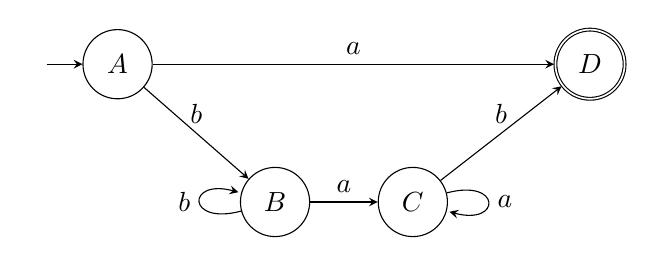
\begin{tikzpicture}[>=stealth,node distance=1.75cm, on grid, auto]

    % Zustände
    \node[state, initial, initial text=] (A) {$A$};
    \node[state, below=of A, xshift=2cm] (B) {$B$};
    \node[state, right=of B] (C) {$C$};
    \node[state, accepting, right=6cm of A] (D) {$D$}; 
    
    % Pfeile
    \path[->]
    (A) edge node[above] {$b$} (B) 
    (A) edge[above] node {$a$} (D) 
    (B) edge [loop left]node[left] {$b$} (B) 
    (B) edge[above] node[above] {$a$} (C) 
    (C) edge[loop right] node[right] {$a$} (C)
    (C) edge node[above] {$b$} (D); 
  
\end{tikzpicture}
\caption{Automat}
\label{tikz}
\end{figure}



\exercise{}
Information hiding \cite{katzenbeisser2016information}.
On the size of pairing-based non-interactive arguments \cite{groth2016size}.


\exercise{}
\begin{enumerate}
\item \ref{tab:länderdaten} Länderdaten
\item \ref{fig:Katze} Katze am Husten
\item \ref{tikz} Automat.
\end{enumerate}

\bibliographystyle{plain}
\bibliography{literature}


% Ende des Dokuments
\end{document}
